\begin{figure}[tb]
    \label{fig:plan-time-n}
    \centering
    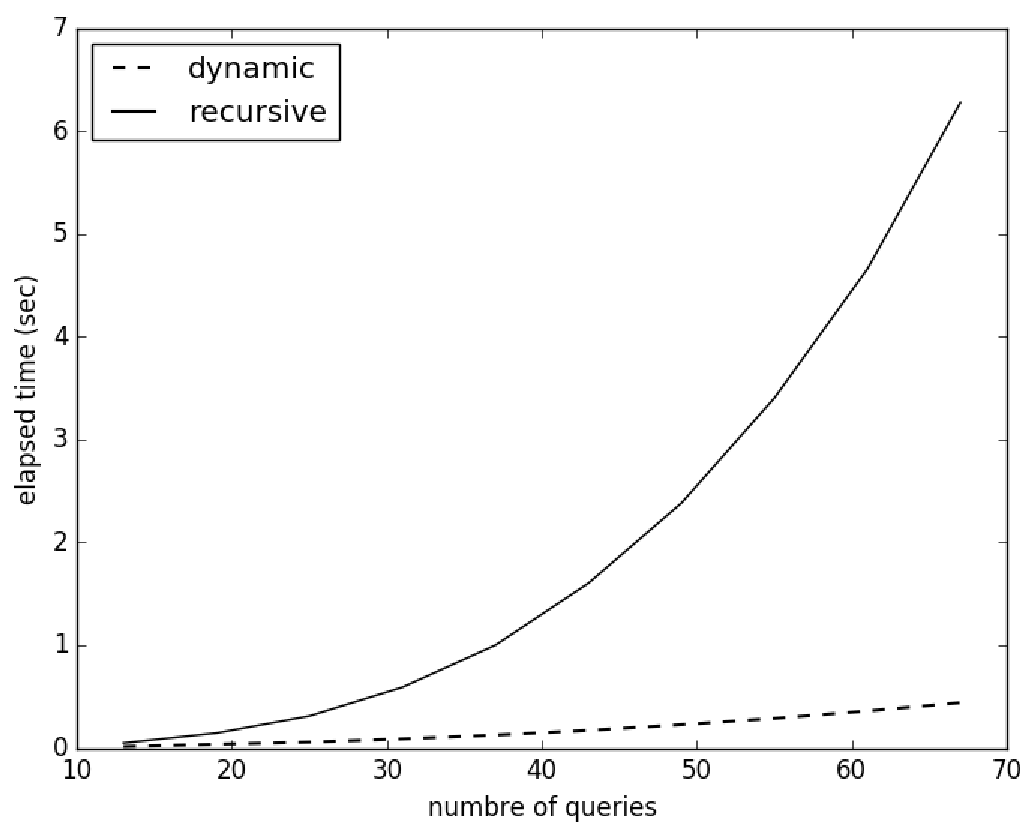
\includegraphics[width=2.5in]{figs/multiquery_runtime.pdf}
    \caption{Optimization time with respect to the number of queries}
\end{figure}


\begin{figure}[tb]
    \label{fig:plan-time-m}
    \centering
    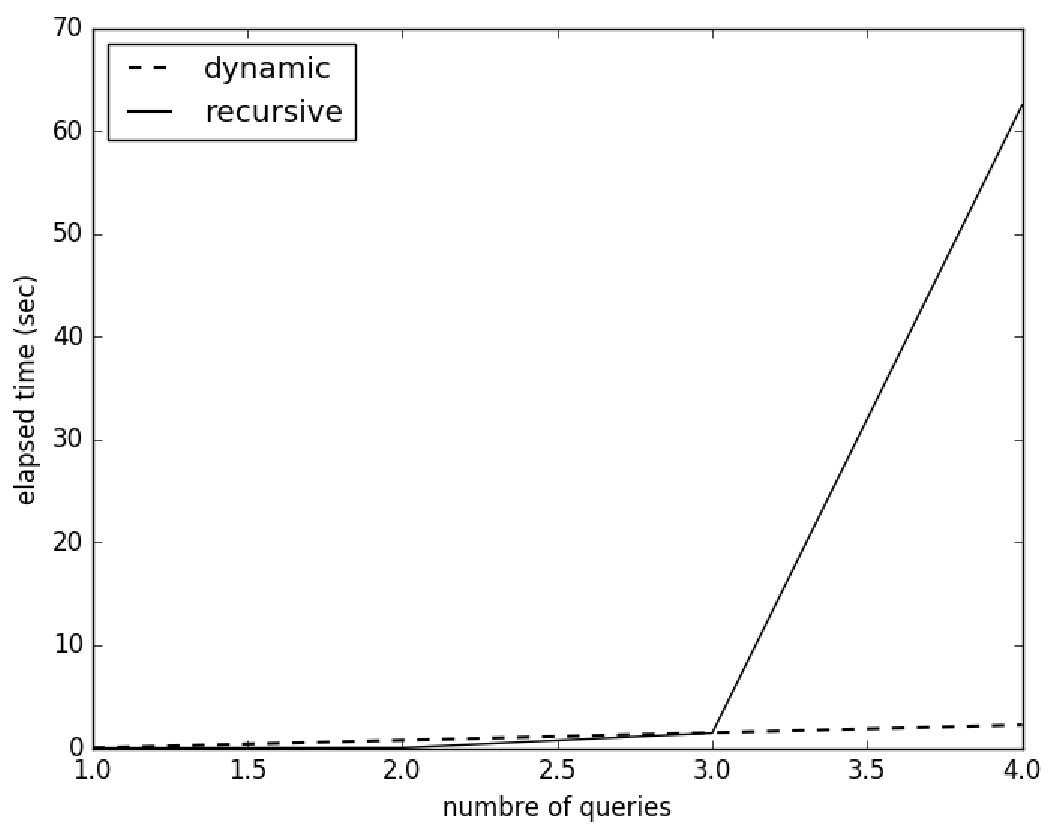
\includegraphics[width=2.5in]{figs/multisnap_runtime.pdf}
    \caption{Optimization time with respect to the number of snapshots}
\end{figure}




\section{Experimental Evaluation}

In order to evaluate our algorithms, we have generated synthetic temporal 
databases.  We have also generated database using the TPCH schema with
~1,000,000 tuples in the main table.  We also created a set of random database
modify, insert and delete updates at 1000 distinct timestamps.  This creates a
temporal database with 1000 timestamps.

To confirm that, without querying at a specific timestamp $q$, the cost is
$\mathcal{O}(q)$ as given by Proposition~\ref{prop:linear-time}, we sampled
100 query timestamps and measured the query answering performance, shown in
Figure~\ref{fig:query-time-no-snap}.  It confirms that the linear-time cost
function is indeed valid in practice.


To evaluate the performance of our {\em optimal} snapshot computation, we
evaluated the recursive formulation given by Section~\ref{sec:recursive}
and the dynamic programming formulation Section~\ref{sec:dynamic}.
Figure~\ref{fig:plan-time-n} and Figure~\ref{fig:plan-time-m} show the
snapshot placement computational time is significantly reduced by dynamic
programming.

To illustrate that the optimal snapshot placement indeed produces the best query
answering performance, we compared the query answering cost of three approaches:
\begin{itemize}
    \item Pick $m$ random timestamps to place the snapshots.
    \item Pick $m$ evenly intervaled timestamps to place the snapshots.
    \item Pick $m$ timestamps computed by dynamic programming.
\end{itemize}
Figure~\ref{fig:comparison} shows that the placements obtained by dynamic
programming clearly beats the other two approaches.

\begin{figure}[tb]
    \label{fig:comparison}
    \centering
    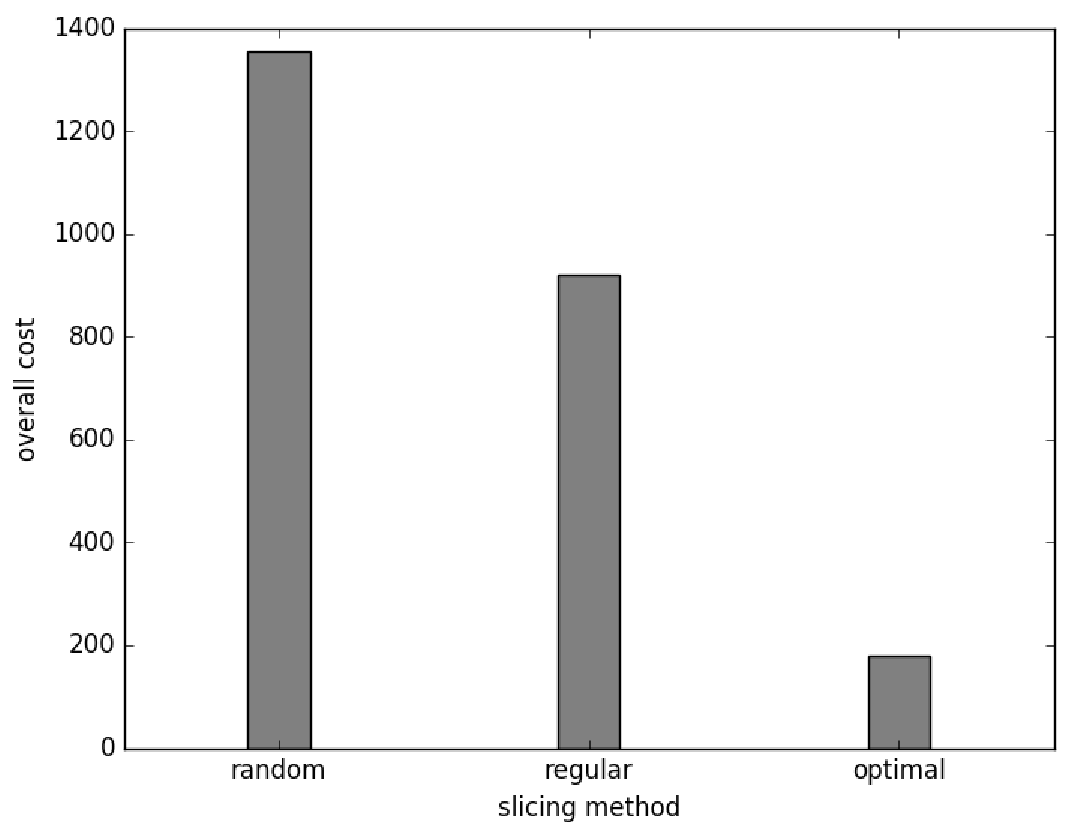
\includegraphics[width=2.5in]{figs/cuts_cost.pdf}
    \caption{Relative query answering cost}
\end{figure}

Finally, we verify the optimality of placing a single snapshot given in
Proposition~\ref{thm:single}.  We set $m=1$, and measured the query answering
cost over different choices of snapshot placement.  Figure~\ref{fig:cost-single}
shows that the optimal placement is at the median of the query times, as
predicated by Proposition~\ref{thm:single}.

\begin{figure}[tb]
    \label{fig:cost-single}
    \centering
    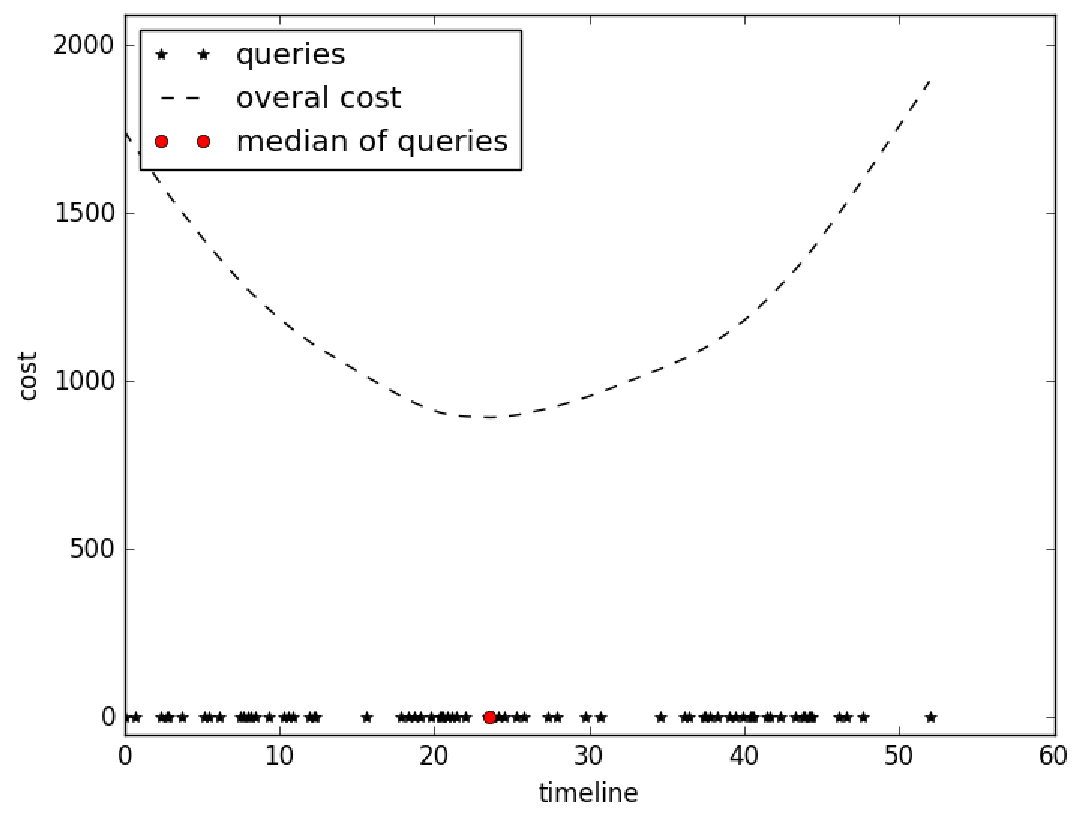
\includegraphics[width=2.5in]{figs/single.pdf}
    \caption{Cost of query answering using a single snapshot over different
    snaptshot timestamps}
\end{figure}

Finally, we demonstrate the query answering performance with increasingly many
snapshots in Figure~\ref{fig:cost-multi}.  It shows that more snapshots will
improve the query performance.  We argue that this is a crucial verification
that our approach will enable efficient temporal query processing for databases
that store the timeline of its tables.

\begin{figure}[tb]
    \label{fig:cost-multi}
    \centering
    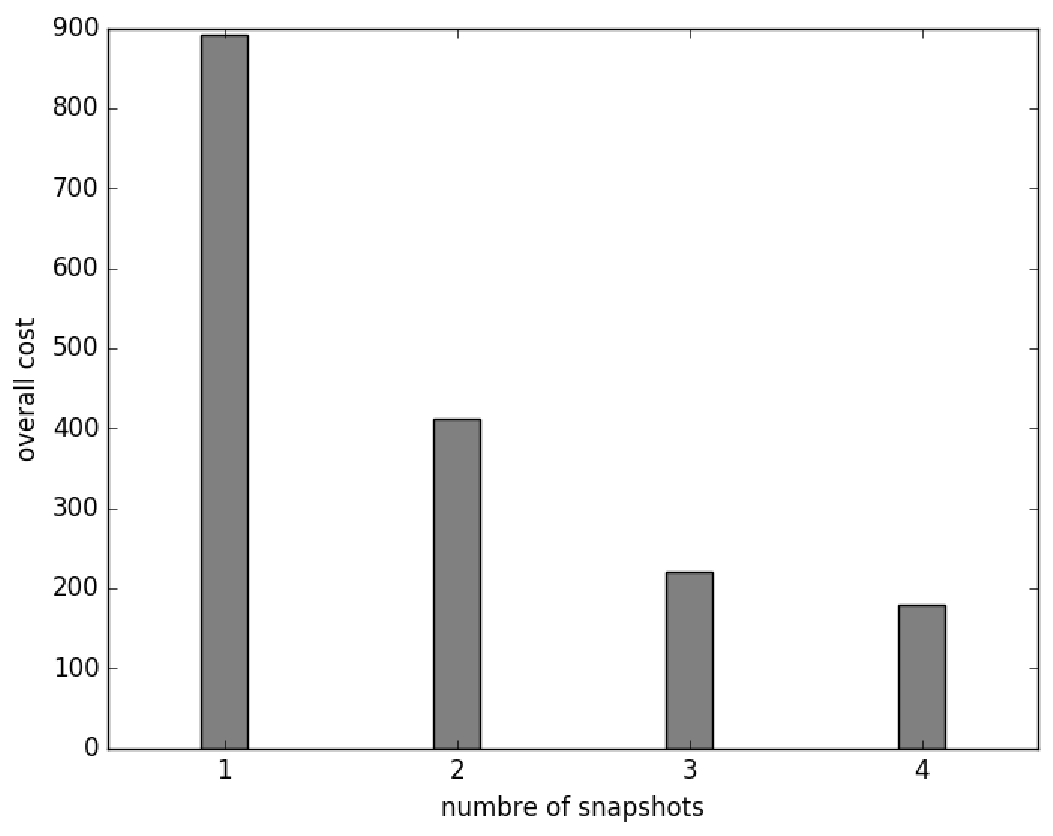
\includegraphics[width=2.5in]{figs/snap_cost.pdf}
    \caption{Query answering cost with increasing number of snapshots}
\end{figure}
